\chapter{Thermostability and Specificity of Ancient Proteins: Assessing the Evidence for Global Trends}

\section{Author Contributions}

Lucas Wheeler, Shion An-Lim, Michael Harms, and Susan Marqusee conceptualized the review and chose specific
topics. Lucas Wheeler and Shion An-Lim conducted the literature review. MJH and SM administered
the project. Michael Harms and Lucas Wheeler generated figures. Lucas Wheeler, Shion An-Lim, Michael Harms, and Susan Marqusee
wrote and edited the manuscript.

\section{Abstract}

Were ancient proteins systematically different than modern proteins?
The answer to this question is profoundly important, shaping how we
understand the origins of protein biochemical, biophysical, and functional
properties. Ancestral sequence reconstruction (ASR), a phylogenetic
approach to infer the sequences of ancestral proteins, may reveal
such trends. We discuss two proposed trends: a transition from higher
to lower thermostability and a tendency for proteins to acquire higher
specificity over time. We review the evidence for elevated ancestral
thermostability and discuss its possible origins in a changing environmental
temperature and/or reconstruction bias. We also conclude that there
is, as yet, insufficient data to support a trend from promiscuity
to specificity. Finally, we propose future work to understand these
proposed evolutionary trends.

\section{Introduction}

Ancestral sequence reconstruction (ASR) has opened a window into the
sequences and properties of ancient proteins \cite{pauling_chemical_1963,harms_analyzing_2010}.
In ASR, a multiple sequence alignment of modern protein sequences
is used to construct a phylogenetic tree and the sequences of ancient
proteins are inferred for specific ancestors on this tree (Figure
1a). By synthesizing the genes encoding these sequences, these reconstructed
ancient proteins can be experimentally characterized. This approach
has yielded an explosion of results in recent years, revealing important
mechanistic insights into the evolution of protein forms and functions
\cite{gaucher_palaeotemperature_2008,voordeckers_reconstruction_2012,bridgham_epistatic_2009,hobbs_origin_2012,akanuma_experimental_2013,akanuma_phylogeny-based_2011,loughran_stability_2014,perez-jimenez_single-molecule_2011,risso_hyperstability_2013,hart_thermodynamic_2014}.

\begin{figure}
\centering 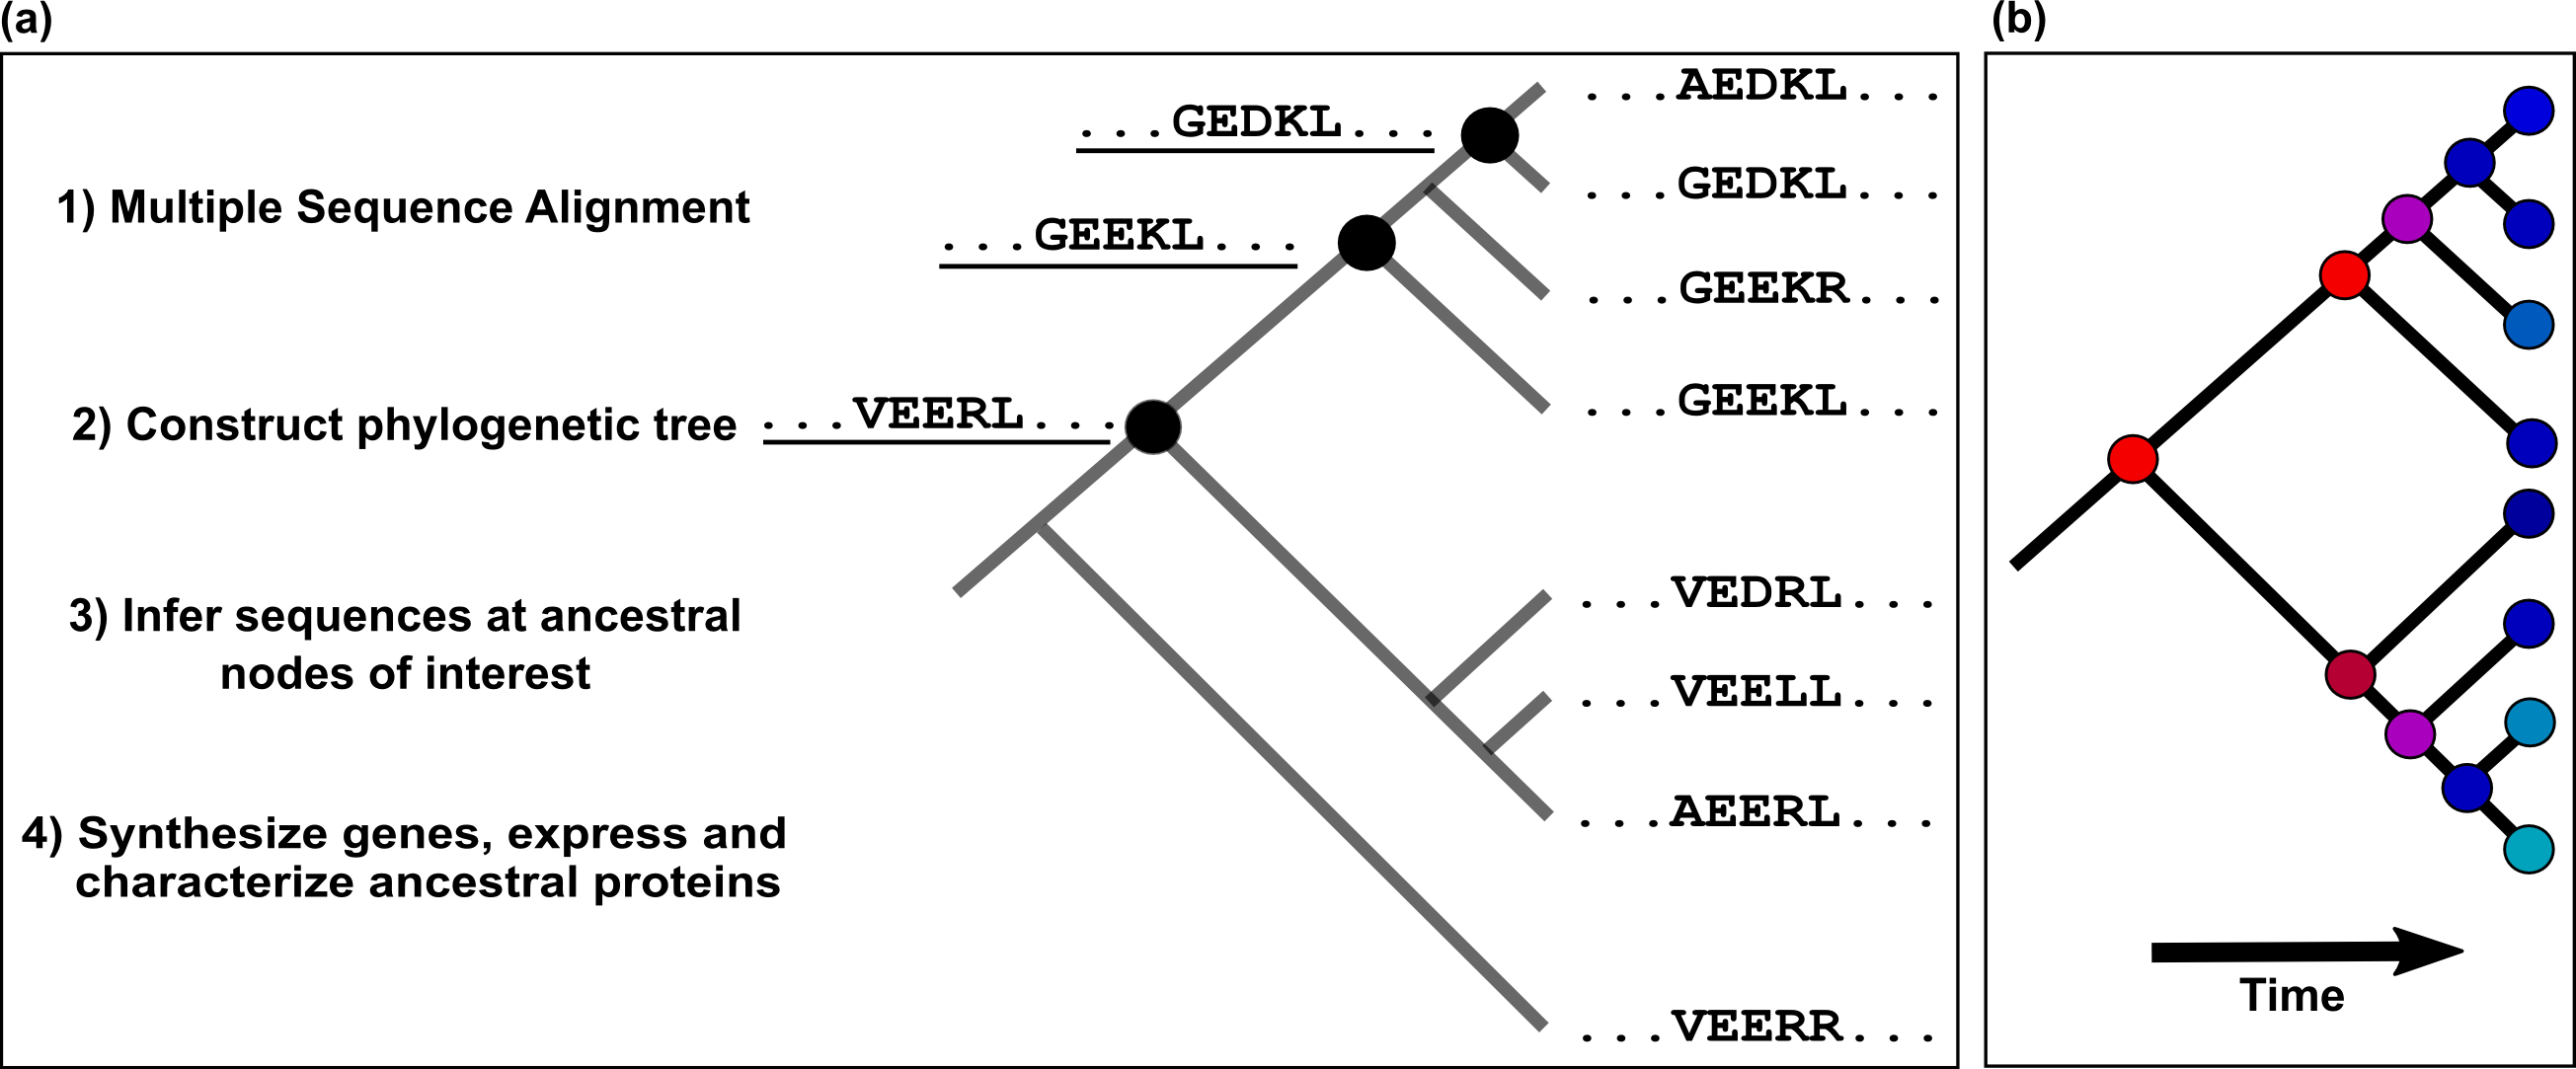
\includegraphics{ch2-fig1} \caption[Ancestral Sequence Reconstruction (ASR) can be used to trace\newline the history
of evolving proteins]{Ancestral Sequence Reconstruction (ASR) can be used to trace the
history of evolving proteins. (a) The ASR pipeline. A multiple sequence
alignment (MSA) of extant sequences of a protein family is generated
using an alignment tool. The MSA is then used to estimate an appropriate
model of sequence evolution and to estimate a phylogenetic tree. The
sequences at ancestral nodes of interest (filled black circles) are
then inferred (underlined) based on the tree and a phylogenetic evolutionary
model. The maximum likelihood sequences are those with the highest
likelihood of generating the known sequences of modern proteins given
the tree and phylogenetic model. Genes encoding the inferred ancestral
proteins can be synthesized, expressed, and purified using standard
molecular biology tools. The properties of the ancestral proteins
can then be experimentally characterized. (b) A phylogenetic tree
showing the evolution of a protein that can vary between two properties\textemdash red
and blue. The last common ancestor was red, but the modern proteins
are blue because of parallel changes along the lineages. This red
ancestor can only be accessed using an approach like ASR.\label{samplefigure}}
\end{figure}

One intriguing possibility is to use ASR to investigate whether ancient
proteins were systematically different in the past, leading to parallel,
directional changes in properties over evolutionary time (Figure
1a). Such trends are inaccessible using comparisons between modern
pro- teins. For example, studies of the modern proteins in Figure
1b would lead one to believe the last common ancestor had a \textquoteleft blue\textquoteright{}
trait. By allowing direct measurement of ancestral properties, ASR
can reveal properties (\textquoteleft red\textquoteright , in this
case) not evident in the modern proteins.

If the evolution of protein properties were directional, it would
provide a new level at which to explain and understand these properties.
This is of deep interest to evolutionary biochemists seeking to identify
the general principles that shape protein evolution. Further, a trend
could mean that sampling evolutionary history would provide access
to qualitatively different proteins \cite{risso_thermostable_2014}
\textemdash{} a boon to engineers looking for proteins with desirable
properties as templates for further engineering \cite{cole_utilizing_2011,whitfield_construction_2015}.

Recent work has suggested two trends over evolutionary time: decreasing
protein stability \cite{gaucher_palaeotemperature_2008} and increasing
specificity \cite{risso_hyperstability_2013}. Particularly for protein
engineers, these trends could be extremely powerful, as high stability
and broad substrate specificity are desirable traits that could be
accessed using ASR. In this review, we review the evidence supporting
and contradicting these trends, as well as the future work required
to test and extend these conclusions.

\section[Reconstructed Precambrian Ancient Proteins]{Reconstructed precambrian ancient proteins exhibit elevated thermostability}

We begin by evaluating evidence from ASR studies that indicate the
deepest ancestors of mesophilic proteins were highly thermostable.
Over billion-year timescales, reconstructed ancestral proteins display
systematically higher thermostability. Reconstructed EF-Tu \cite{gaucher_palaeotemperature_2008},
thioredoxin \cite{perez-jimenez_single-molecule_2011}, DNA gyrase
\cite{akanuma_phylogeny-based_2011}, nucleotide diphosphate kinase
\cite{akanuma_experimental_2013}, and $\beta$-lactamase \cite{risso_hyperstability_2013}
all exhibit melting temperatures (T$_{m}$) far higher than their
extant descendants. Some have argued that this is a universal trend
\cite{risso_thermostable_2014} and have interpreted this as evidence
for an ancient, hot environment \cite{gaucher_palaeotemperature_2008}.
The evidence, however, is not completely universal, as reconstructed
RNase H along a mesophilic lineage gives a relatively flat trend in
stability over similar time scales \cite{hart_thermodynamic_2014}.

One difficulty in comparing these studies is that different proteins
have different absolute requirements for stability. For example, the
T$_{m}$'s of EF-Tu bacterial homologs are generally $\sim$2 $^{\circ}$C
above the environmental temperature (T$_{env}$), while the T$_{m}$s
of RNase H are $\sim$30 $^{\circ}$C above T$_{env}$. As a result,
T$_{m}$s between protein families are not directly comparable. One
way to overcome this challenge is to convert the measured T$_{m}$
of each protein to an estimate of T$_{env}$, as T$_{m}$ often correlates
with the growth temperature of the organism from which it was derived
\cite{gromiha_important_1999}. In most cases, this correlation arises
to maintain stability above some critical threshold \cite{taverna_why_2002}.
Empirically, T$_{m}$ generally rises by $\sim$1 $^{\circ}$C per
1 $^{\circ}$C of T$_{env}$, with an offset reflecting the required
stability of the protein (e.g. 2 $^{\circ}$C for EF-Tu and 30 $^{\circ}$C
for RNase H) \cite{gromiha_important_1999}. This correlation has
been directly established for three of the proteins above \textemdash{}
EF-Tu, DNA gyrase and RNase H \cite{gaucher_palaeotemperature_2008,akanuma_experimental_2013,hart_thermodynamic_2014}
\textemdash{} and holds generally for many other proteins \cite{gromiha_important_1999}.

When placed on the T$_{env}$ scale, reconstructed proteins report
an elevated environmental temperature $\sim$3 billion years ago,
though with significant scatter. Figure 2a shows the estimated T$_{env}$
over time for 17 ancestors of proteins found in the lineages leading
to mesophilic $\textit{E. coli}$. A total least-squares fit to the
data reveals a highly significant negative slope that explains 75\%
of the variation in the data (R$^{2}$ = 0.75). In contrast, the estimated
T$_{env}$ over time for ancestors leading to thermophile $\textit{T. thermophilus}$
exhibits a slope statistically indistinguishable from 0 ( Figure 2b).
When taken in aggregate, these data support the hypothesis that the
deepest ancestors had stabilities similar to proteins from modern
thermophiles. While these data focus on the $\textit{E. coli}$ and
$\textit{T. thermophilus}$ lineages, their deepest ancestors are
shared both with each other and with most modern bacteria, thus suggesting
a global transition away from ancient thermostability, at least along
mesophilic lineages. It is not clear from these sparse, lineage-specific
data whether mesophilicity evolved in parallel along many lineages
or whether it evolved on a few key, early ancestral branches.

\begin{figure}
\centering 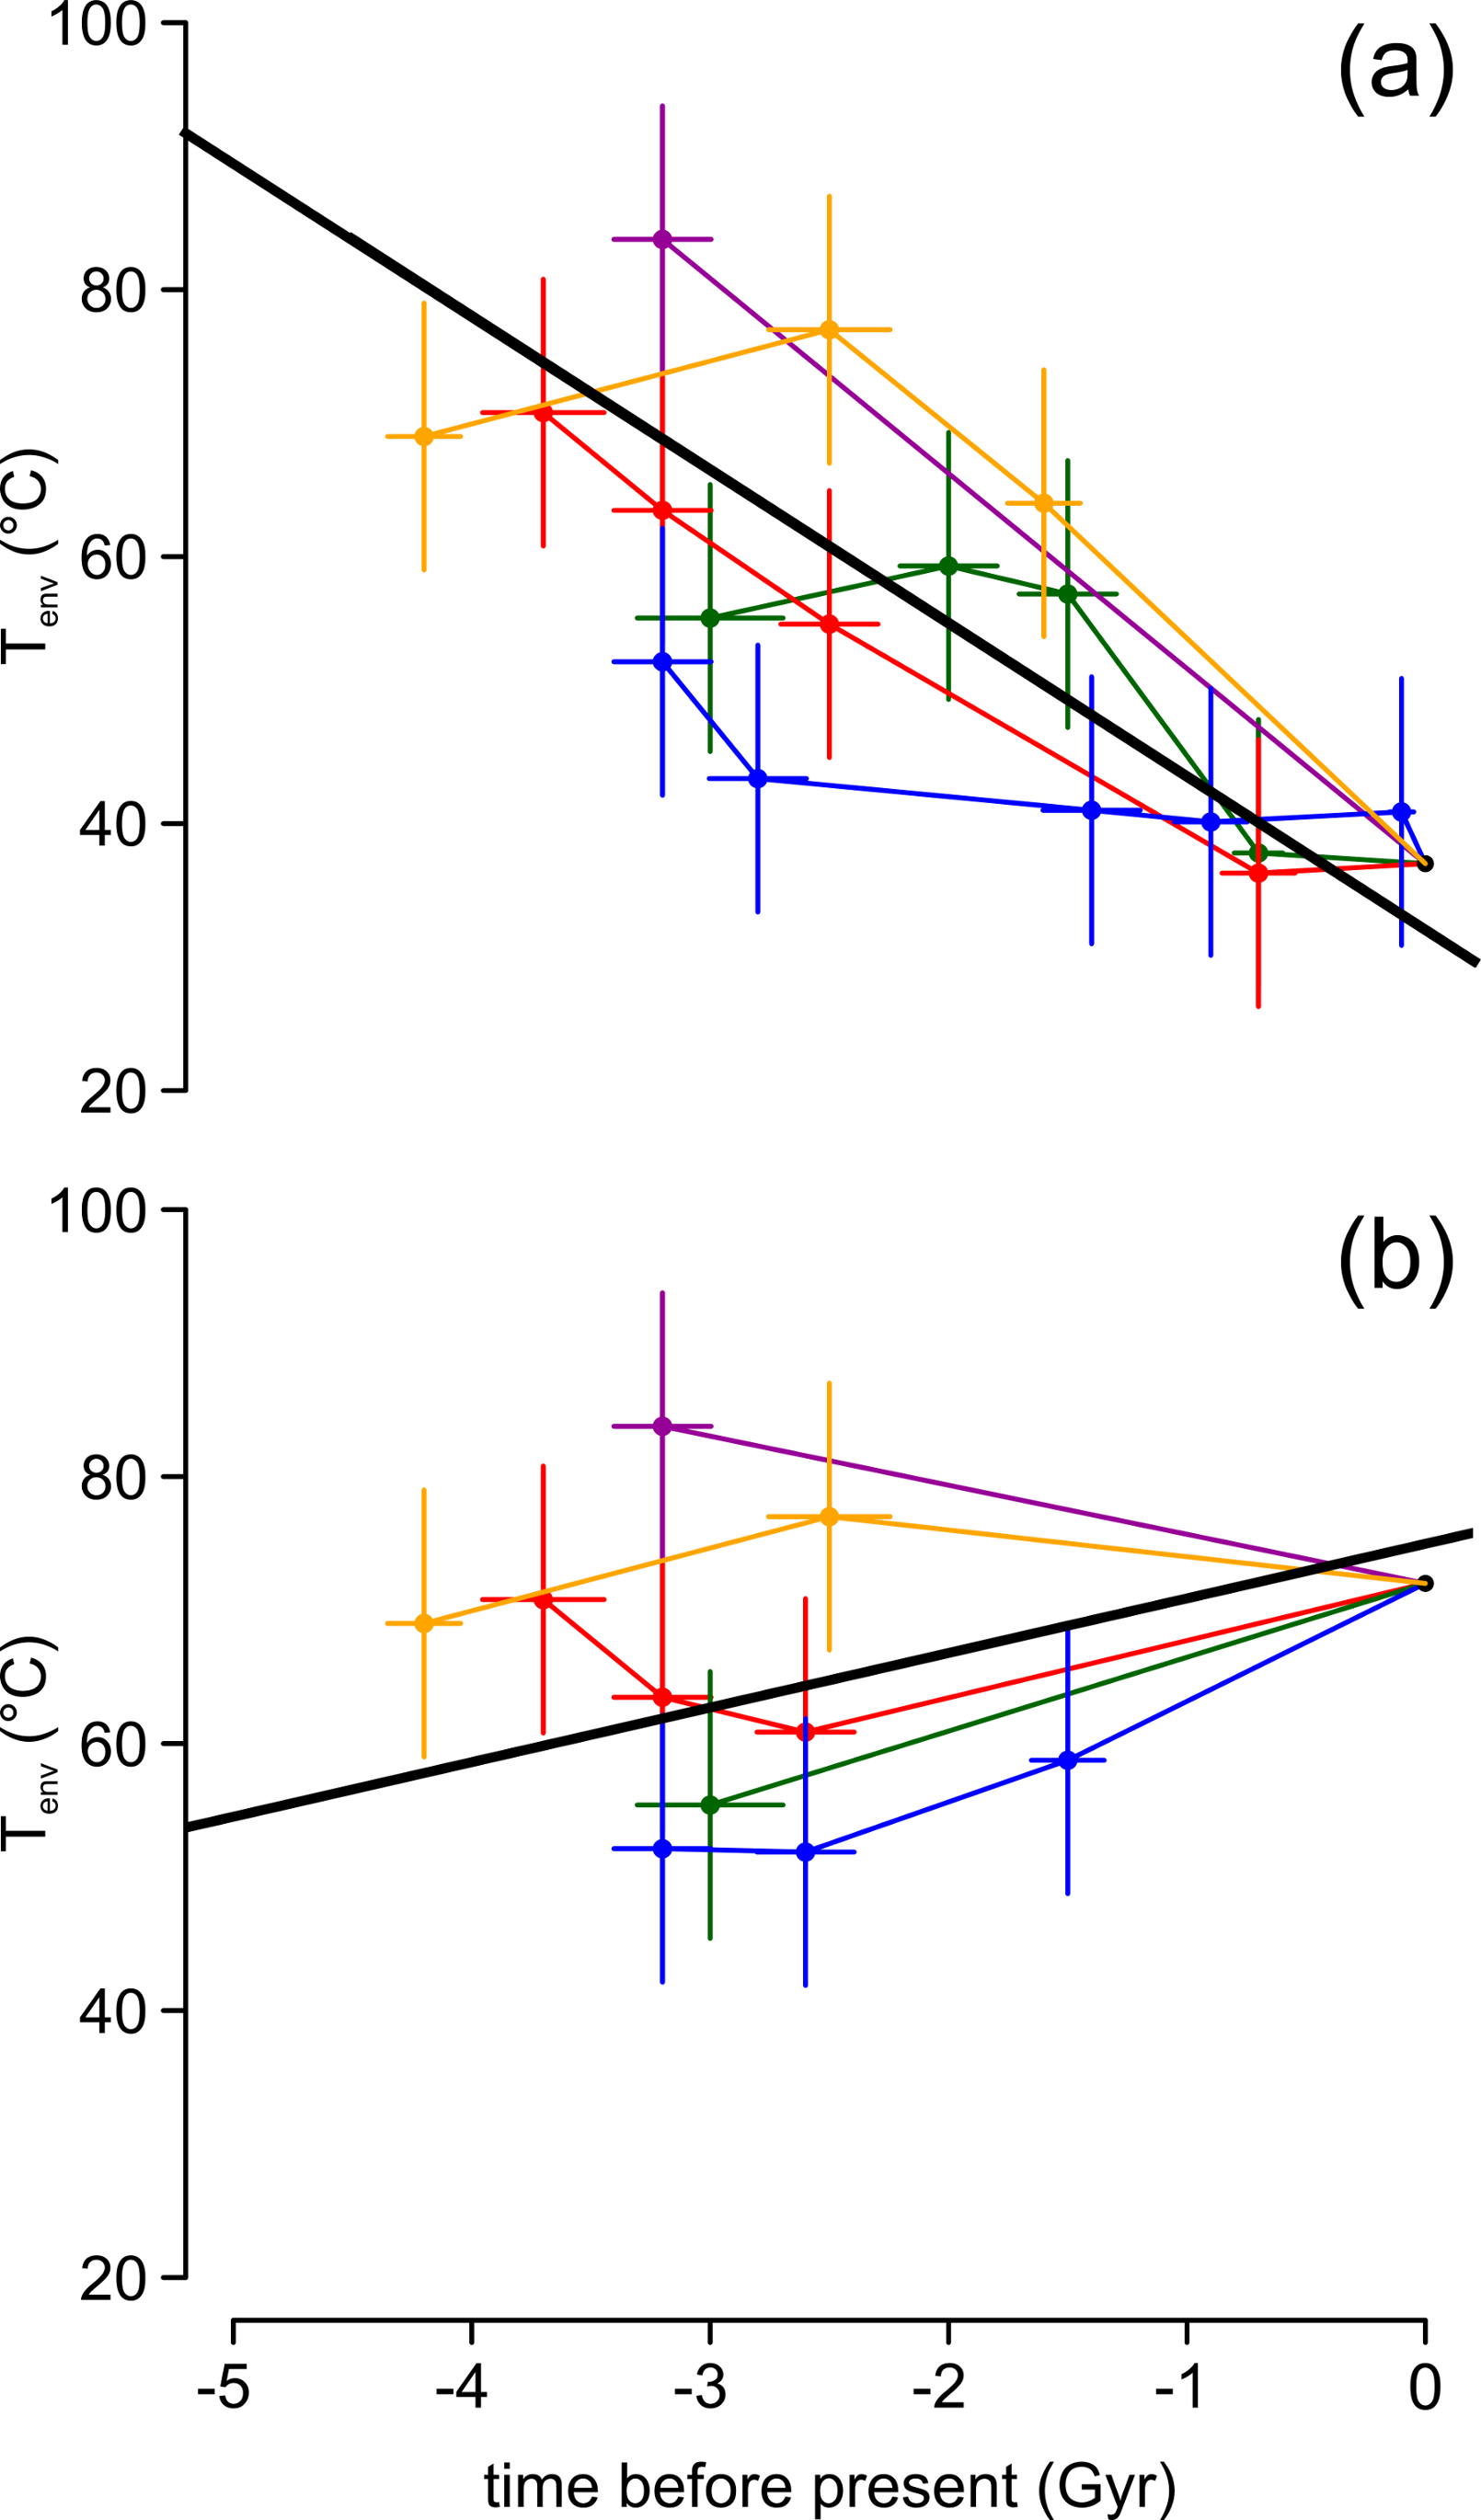
\includegraphics{ch2-fig2-smaller} \caption[Ancient Reconstructed Ancestors Exhibit Elevated\newline Thermostability]{Ancient reconstructed ancestors exhibit elevated thermostability.
Estimated environmental temperatures experienced by proteins on lineages
leading to (panel a) \textit{E. coli} or (panel b) \textit{T. thermophilus}.
Point/line series indicate individual protein families: EF-Tu (red),
thioredoxin (orange), $\beta$\textendash lactamase (green), RNase
H (blue), and nucleotide diphosphate kinase (purple). Measured melting
temperatures for ancestors that give rise to E. coli proteins were
mined from published literature \cite{gaucher_palaeotemperature_2008,akanuma_experimental_2013,perez-jimenez_single-molecule_2011,risso_hyperstability_2013,hart_thermodynamic_2014}.
These were then converted to estimates of T$_{env}$ using measured
relationships \cite{gaucher_palaeotemperature_2008,akanuma_experimental_2013,hart_thermodynamic_2014}
or by adding an offset determined by the difference in T$_{m}$ and
T$_{env}$ for the \textit{E. coli} (panel a) or \textit{T. thermophilus}
homologs (panel B). Time estimates were drawn from original publications
or estimated from Battistuzzi et al. \cite{battistuzzi_genomic_2004}.
Time errors are standard errors. T$_{env}$ standard errors were set
to $\pm$ 10 $^{\circ}$C to account for uncertainty in T$_{m}$ and
the T$_{m}$/T$_{env}$ correlation. (This is a conservative estimate:
when measured for NDK, RNase H, and EF-Tu \cite{gaucher_palaeotemperature_2008,akanuma_experimental_2013,hart_thermodynamic_2014}
, the T$_{m}$ the standard error was $<$5 $^{\circ}$C and the T$_{m}$
to T$_{env}$ variance was $<$5 $^{\circ}$C.) Black line is a fit
determined by total linear regression. To find the standard deviation
of fit slopes, we generated 1000 pseudo datasets sampled from the
time and T$_{env}$ uncertainties. For E. coli, the fits reject a
slope = 0 (p = 3 $\times$ 10$^{-8}$). For \textit{T. thermophilus},
the fits fail to reject a zero slope (p = 0.45).\label{samplefigure}}
\end{figure}


\section{Trends in Thermostability Are Complex}

While ASR studies suggest that the most ancient proteins were highly
thermostable, they do not support a smooth trend in thermostability
over time. Ancestors exhibit extensive random scatter to the proposed
trend. Such variation is expected as, over more recent timescales,
protein stability fluctuates in response to neutral drift or adaptation
in apparently random fashion \cite{hobbs_origin_2012,loughran_stability_2014,malcolm_ancestral_1990,dasmeh_positively_2013,gong_stability-mediated_2013}.
The observed variation may also reflect uncertainty in the reconstruction,
multiple heterogeneous environments experienced by ancient organisms,
or uncertainty in the map between T$_{m}$ and T$_{env}$.

This scatter extends to the mechanism of stabilization. A recent study
of the evolution of thermostability in RNase H revealed that the thermodynamic
mechanism of stabilization for the ancestral proteins could fluctuate,
even as the T$_{m}$s of the proteins varied smoothly \cite{hart_thermodynamic_2014}.
This indicates that, even while under selection to maintain stability
in a given environment, proteins are free to accumulate mutations
to access alternate mechanisms of stabilization. Practically, studying
multiple ancestors may reveal new sequence and thermodynamic determinants
of stability. Although thermostability and the mechanism of stabilization
appear to change independently for RNase H, the generality of this
result for other proteins remains unknown.

Finally, these ASR studies generally used small, monomeric, and well-behaved
proteins. Although such simple proteins may be representative of the
first proteins to arise, studies on a greater diversity of protein
families will reveal whether observed trends are applicable to the
entire proteome.

\section{Can Reconstruction Errors Inflate Ancestral Thermostability?}

While existing data are suggestive, further work must be done to test
the hypothesis of ancient thermostability. The primary concern is
that ancestral proteins are statistical reconstructions that cannot
be directly verified. Even with good statistical support, it is unlikely
that the reconstructed ancestor will have the exact sequence of the
true ancestral state. Addressing and understanding this uncertainty
will be critical for establishing or refuting the hypothesis that
the earliest proteins were thermostable.

High stability is unlikely to arise from random errors in the reconstruction.
To account for uncertainty, ASR studies have generated different versions
of ancestral sequences to assess the robustness of the measured stability
to phylogenetic errors. For example, Hart et al. measured ten alternate
sequences of a $\sim$3 billion year-old ancestor and found a T$_{m}$
of 76.7 $\pm$ 2 $^{\circ}$C (compared to 68.0 $^{\circ}$C of RNase
H from $\textit{E. coli}$) \cite{hart_thermodynamic_2014}. Using
such approaches, many sources of random error have been investigated:
uncertain tree topology \cite{gaucher_palaeotemperature_2008,akanuma_experimental_2013,groussin_toward_2015,hanson-smith_robustness_2010},
alternate evolutionary models \cite{akanuma_robustness_2015}, choice
of reconstruction method \cite{hobbs_origin_2012,hanson-smith_robustness_2010},
different amino acid frequencies \cite{gaucher_palaeotemperature_2008},
and reconstruction ambiguity \cite{gaucher_palaeotemperature_2008,akanuma_experimental_2013,risso_thermostable_2014,hart_thermodynamic_2014,bar-rogovsky_assessing_2015}.
In all such studies, the properties of the ancestors have proven robust
to uncertainty.

Of bigger concern are sources of systematic error in ASR \textemdash{}
in particular, a bias towards elevated stability for deeper ancestors
\cite{williams_assessing_2006,bershtein_intense_2008,pollock_amino_2012,goldstein_nonadaptive_2015}.
Some have argued that ASR could be biased towards consensus sequences,
which may lead to an increase in stability \cite{bershtein_intense_2008,gaschen_diversity_2002,kothe_ancestral_2006}.
Simulations have also suggested that maximum likelihood (ML), the
most popular form of ASR, may give rise to artificially elevated stability
\cite{williams_assessing_2006}. If different stabilizing mutations
accumulate along different lineages, ML may incorrectly incorporate
all of the stabilizing mutations, creating an artificially stable
ancestor. There is also concern that variable amino acid distributions
and mutation rates can alter reconstructions \cite{pollock_amino_2012,goldstein_nonadaptive_2015}.

There have been some limited experimental tests of these computational
predictions of bias. Comparisons between ancestral and consensus sequences
have shown distinct statistical and functional properties \cite{akanuma_experimental_2013,akanuma_phylogeny-based_2011,cole_utilizing_2011,risso_phenotypic_2014}.
This suggests that any consensus bias that exists must be subtle.
Other work has indirectly addressed this concern - the molecular basis
of stability fluctuating over evolutionary time in the RNase H family
is not consistent with bias arising from a single, convergent stabilization
mechanism \cite{hart_thermodynamic_2014,williams_assessing_2006}.

Important experiments remain. One test would be a systematic comparison
of ancestors reconstructed using both ML and an alternative, Bayesian,
method. A Bayesian reconstruction averages over uncertainty; therefore,
it is not expected to have the same stability bias as ML reconstructions
\cite{williams_assessing_2006}. Observing high thermostability in
ancient Bayesian ancestors would be strong evidence that thermostability
is not an artifact of the ML method. The experiment is not perfect,
however, as Bayesian ancestors have more errors than ML ancestors
as a result of incorporating uncertainty \cite{hanson-smith_robustness_2010}.
Because of this, they may not accurately reflect the ancestral state.
For example, one study found that a Bayesian ancestor had fundamentally
different folding properties than the ML ancestor or any modern protein
in the family \cite{hobbs_origin_2012}, consistent with a poor reconstruction.

Another test for bias would be to study the thermostability of reconstructed,
recent ancestors of rapidly evolving proteins with known mesophilic
ancestral environments. A rapidly evolving protein will accumulate
similar amounts of mutations relative to the deep ancestors studied
to date, albeit on a much shorter timescale. If ML reconstructions
lead to biased stability, we would predict that recent ancestors of
rapidly evolving proteins would exhibit erroneously elevated stability.

\section{A Trend from Promiscuous to Specific is Not Yet Established}

Another proposed trend is that proteins have, on average, changed
from lower to higher specificity over deep evolutionary time \cite{risso_hyperstability_2013,risso_thermostable_2014}.
This stems from the idea that low specificity proteins \textemdash{}
particularly enzymes \textemdash{} were important for the ability
of primordial organisms to perform diverse chemical processes with
a limited proteome \cite{jensen_enzyme_1976} (Figure 3a). It is also
well established that increased specificity often follows gene duplication
via subfunctionalization from a multi-functional or promiscuous ancestral
protein \cite{lynch_probability_2000,conant_turning_2008} (Figure
3b). Given these considerations, proteins may, on average, increase
in specificity over time.


\begin{figure}
\centering 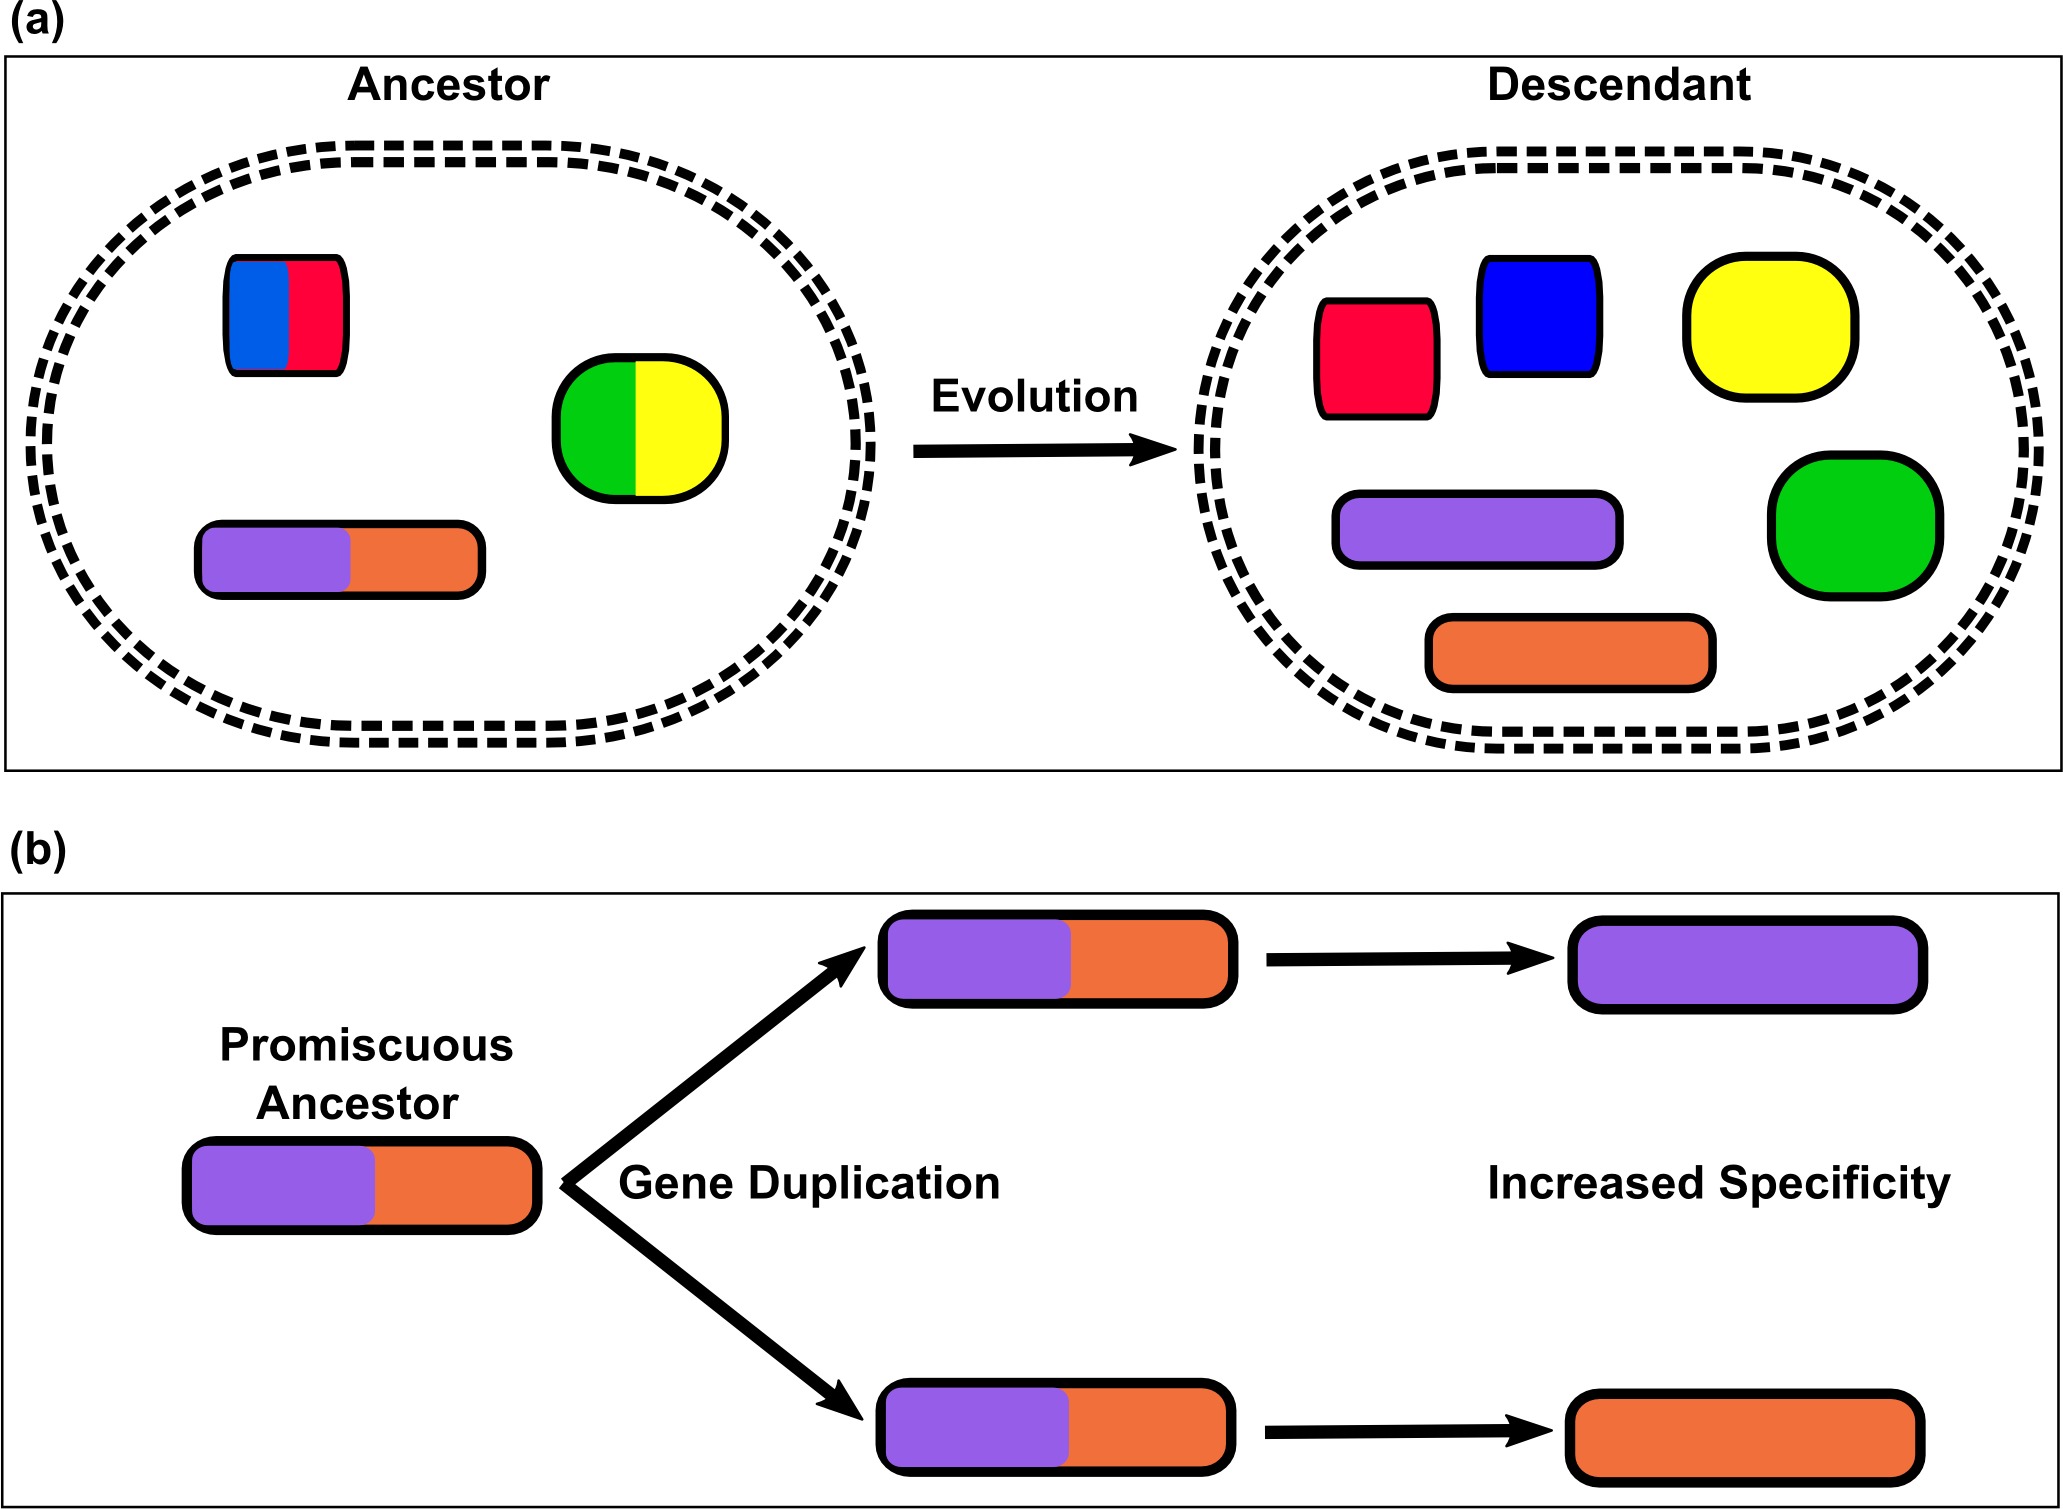
\includegraphics{ch2-fig3} \caption[Models for increased specificity of proteins over time]{Models for increased specificity of proteins over time.(a) Large
dotted ellipses denote cells. Small ellipses are proteins, colored
by their specificity. Because early proteomes were presumably smaller
than modern proteomes, it has been proposed that ancient proteins
had to be promiscuous to achieve all the necessary chemistry. As organisms
evolved, their proteomes expanded, allowing each protein to become
more specific. (b) Higher specificity (subfunctionalization) is one
of the possible outcomes of a gene duplication event. A gene encoding
a low-specificity ancestral protein duplicates. Its descendants can
then gain specificity and lose the promiscuous trait.\label{samplefigure}}
\end{figure}

To date, few attempts have been made to investigate the specificity
of the deepest ancestors. One recent study found that an ancestral
$\beta$-lactamase was both promiscuous and less efficient than its
descendants \cite{risso_hyperstability_2013}. Likewise, a study of
RuBISCO found a promiscuous and inefficient ancestor, though this
may be an artifact of poor reconstruction \cite{ma_molecular_2016}.
Other studies have determined the activities of ancient proteins,
but not their specificity \cite{hobbs_origin_2012,akanuma_experimental_2013}.
On the basis of these data, it is difficult to make solid conclusions
about specificity trends; more measurements of ancestral specificity
are warranted.

The second model \textemdash{} gene duplication followed by subfunctionalization
\textemdash{} could conceivably operate continuously through evolution,
leading to progressively higher specificity proteins over all evolutionary
timescales (Figure 3b). Studies of the evolution of specificity for
ancestors from the last $\sim$500 million years suggest, however,
that on average, proteins do not tend towards higher specificity over
time. Some promiscuity-to-specificity transitions have been identified
\cite{risso_hyperstability_2013,eick_evolution_2012,boucher_atomic-resolution_2014,wouters_despecialization_2003,wilson_using_2015}.
However, other studies have found switches between two high-specificity
states \cite{mckeown_evolution_2014,clifton_ancestral_2016}, evolution
through a less-specific intermediate \cite{sayou_promiscuous_2014,aakre_evolving_2015,howard_ancestral_2014},
and even decreased specificity over time \cite{chinen_evolution_2000}.

This complexity likely arises because specificity is, at minimum,
a bimolecular process that involves both the protein and its target.
Further, constraints placed by the architecture of the larger system
into which the proteins are embedded have been shown to shape specificity
\cite{howard_ancestral_2014,chinen_evolution_2000,peleg_evolution_2014,kim_inhibitory_2012,hong_molecular_2014,vos_breaking_2015,ernst_coevolution_2010,stiffler_pdz_2007}.
For example, bioinformatic analyses have revealed that protein components
of higher-complexity regulatory modules tend to possess lower specificity
than those in simpler modules \cite{stewart_evolution_2013}. We therefore
believe that it will be difficult to resolve a global evolutionary
trend from lower to higher specificity.

\section{Conclusions}

A number of ASR studies are starting to reveal a consistent pattern
of elevated thermostability for the deepest ancestors. This trend
of decreasing thermostability among mesophilic lineages is not smooth,
involving fluctuations in both T$_{m}$ and mechanism of stabilization.
Whether this reflects a real evolutionary signal or simply an artifact
of the reconstruction method remains to be seen. From an engineering
perspective, a ML reconstruction of an ancient ancestor appears to
be a reasonable strategy for generating a thermostable, thermophilic-like
protein that differs from a simple consensus sequence. This approach
is not guaranteed \textemdash{} for example, reconstructed RNase H
displays non-thermophilic-like thermostability $\sim$3 billion years
in the past \textemdash{} however, on average, deep ancestral proteins
appear to be more stable than their modern counterparts. We should
also note that these are deep trends, and thus we would not predict
recent ancestors to exhibit any detectable trend in stability, consistent
with recent studies \cite{hobbs_origin_2012,loughran_stability_2014,dasmeh_positively_2013}.

Information about the specificity of deep ancestral proteins remains
sparse and will thus require further investigation. Studies of more
recent proteins indicate that multiple modes of specificity evolution
can be at play, suggesting a lack of general trends.

Protein evolution is often viewed as a random, microscopically-reversible
trajectory along a fitness landscape. A global trend would suggest
that the fitness landscape changed in a systematic way, even while
microscopic reversibility held. Such systematic changes in fitness
landscape would, in turn, shape the pathways taken by proteins and
provide another level at which to understand the emergence of new
properties. ASR studies are hinting at a change in fitness landscape.
This may help us, at a broad brush level, gain insight into the origins
of protein features and properties.

\section{Bridge to Chapter III}

In this chapter, the current evolutionary biochemistry literature
was reviewed to assess the available evidence for broad evolutionary
trends in protein properties. Two highly-referenced examples of trends
were analyzed: the hypothesis that proteins have undergone a gradual,
monotonic decrease in thermal stability over long time scales and
the assertion that proteins generally become more specific over time
as proteomes become increasingly complex. The conclusion was drawn
that there is some evidence to support a long-term decreasing trend
in thermostability. However, there is still relatively sparse information
available. More experiments will need to be targeted toward addressing
this question to establish firm conclusions. With regard to the evolution
of specificity, this chapter concluded that there is vastly insufficient
evidence to draw strong conclusions. Furthermore, unlike decreases
in thermostability there is no unifying theoretical reason to expect
global, parallel increases in specificity over time. This chapter
established the need for further experimentation and more complete
theories to address the issue of global trends in protein evolution.
Chapter III addresses trends in a specific biochemical feature during
the evolution of an entire protein family. An interesting observation
is made regarding the evolutionary lability of this feature and its
underpinnings at the amino acid level. 


